\chapter{Fundamentals}
\label{chap:methods}

\todo{FRAGE: Diagramme aus tensorboard, wie viel Glätten?}

\todo{replace taxonomy with actual chapters: "functions to improve behaviour" - policy, value fnc, q-fnc; TD: qlearning, sarsa; exploration vs exploitation: all strategies}

\todo{ML chapter with: supervised, unsupervised, RL}
\todo{libs vorstellen und dann sagen für openai entschieden: openai baselines, stable baselines, openai spinning up, RLlib}
\todo{hyperparams chapter}
\todo{if more pages needed: Neural Network basics: neurons, weights, bias, batch, normalization, regularization, activation function, layers, etc. + deep + recurrent, cnn, etc. feed forward, backpropagation, bellman equation, TD(Qlearning, SARSA) and Monte-Carlo (thorough)}
\todo{boltzmann exploration, (more policy strategies?}
\todo{can add actuall algorithms to fill up space}
\todo{more/similar DRL algorithms, e.g. explicit TRPO, DDPG, A2C, A3C, Rainbow, Genetic Algorithms? ONE-STEP, MULTI-STEP }
\todo{add equation for everything}
\todo{summary for each chapter?}
\todo{regression, classification}
\todo{svm, trees, auto-encoder?}
\todo{was first chapter, review this all}


In this chapter, the fundamentals of Reinforcement Learning (RL) are introduced. First, the basics of RL is explained, such as the definition of key terms and concepts, and notations, if any. Followed by basic RL-algorithms and finally, depp algorithms.. \todo{rewrite when done}
 This is necessary to understand the deep algorithms, that are used later on in the experiments in chapter \ref{chap:experiments}, namely, \nameref{ssec:dqn} (DQN), \nameref{para:ddqn} (DDQN), \nameref{ssec:ppo} (PPO) and \nameref{ssec:reinforce}.

\section{Reinforcement Learning}
\label{sec:rl}

\subsection{Background}
Reinforcement Learning is one of the three main paradigms in \textit{Machine Learning}. These paradigms use algorithms that learn from experience to enhance the performance in their respective tasks \cite{mohri2018foundations}. The remaining paradigms are \textit{Supervised Learning} and \textit{Unsupervised Learning}. In the former paradigm, the \textit{learner} learns from training data, that is \textit{labeled}. This means that the training data has been augmented with additional information, such as output labels of the correct \textit{class} in the case of a classification problem, i.e. in a training set consisting of various animal images, the output labels would be the name of the animal, for each image. The learner learns to association the training data with their respective labels and applies the knowledge to unseen data, to map them to the correct labels. The latter paradigm also uses predefined training data, however, it does not use labels. Thus, it is not clear what to look for and there is also no feedback, since there are no labels associated with the training data. However, Unsupervised Learning can be used to identify patterns in unstructured data, e.g. clustering \cite{alzubi2018machine}.

In Reinforcement Learning the learner, or rather \textit{agent} in that context, learns from a \textit{reward}, that is acquired by interacting with an \textit{environment}, by trial-and-error. The learner is observing a \textit{state} in an environment, at a specific time, and is performing an \textit{action}, based on the information it has. Finally, the agent obtains a reward for its action and the environment transitions into its next state. This interaction is known as the agent-environment interaction and is illustrated in Figure \ref{fig:agent_env_loop}. 

The aim of the agent is to maximize the expected cumulative reward from the environment. This is done, by continuously interacting with the environment in an endless loop, until a termination condition is reached. A single transition in the loop is usually called an \textit{episode}. The agent does not know in advance, what rewards it can expect for its action in a given state. It has to learn those by trial-and-error, thus exploring the environment and finding out which actions lead to the highest rewards. Based on the environment, an action might not only influence the immediate reward, but distant rewards as well, due to state transitions after each episode. This process can be described as a finite Markov Decision Process (MDP) \cite{richardsutton2018}.

\begin{figure}[H]
  \centering
  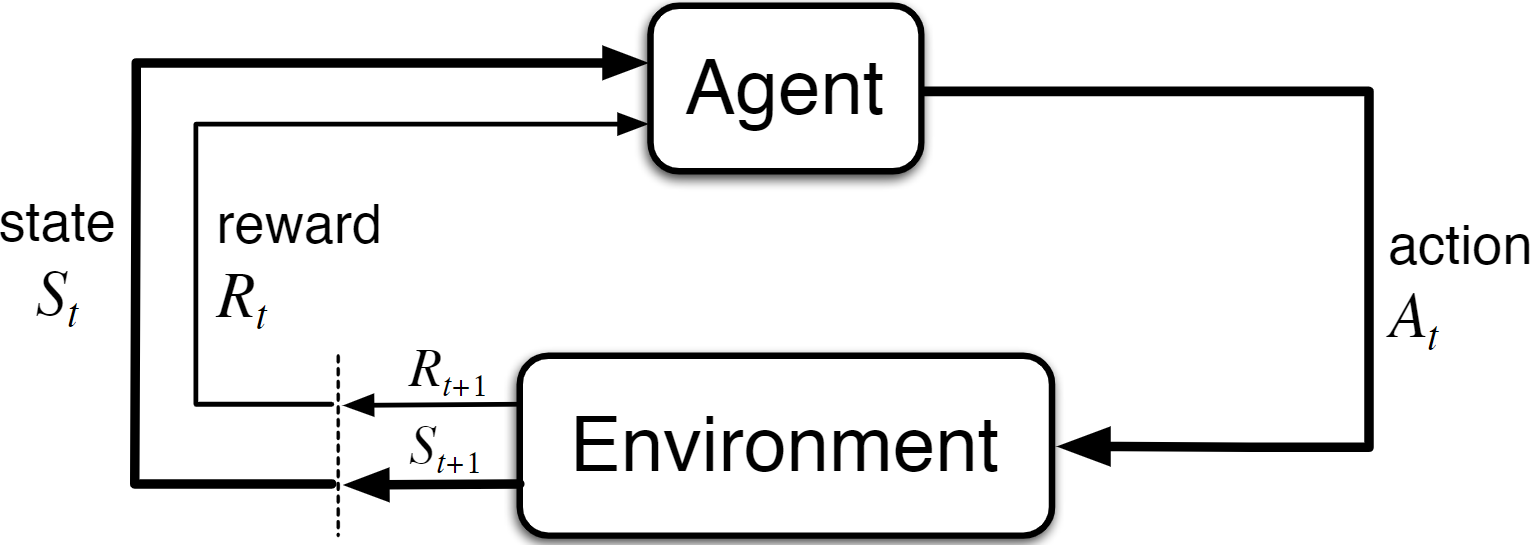
\includegraphics[scale=0.25]{images/rl_interaction}
  \caption[Agent-environment interaction]{Agent-environment interaction. The agent performs an action $A_t$ in state $S_t$ of an environment. The environment transitions into the successor state $S_{t+1}$ at the end of the episode and the agent received a reward $R_{t+1}$ for his action and the new state. This procedure is repeated until a termination condition is reached. Source: Reprinted from \cite[p.48]{richardsutton2018} }
  \label{fig:agent_env_loop}
\end{figure}


\paragraph[MDP]{Markov Decision Process}
\label{para:mdp}
A MDP can be formalized as a tuple \(\langle \mathcal{S, A, P, R, } \gamma \rangle\), where \(\mathcal{S}\) and \(\mathcal{A}\) are finite sets of states and actions, respectively. \(\mathcal{P}\) is a state transition probability matrix, where the probabilities for all states $\mathnormal{s}$ with action $\mathnormal{a}$ to all successor state $\mathnormal{s'}$ is stored. \(\mathcal{R}\) is a function to calculate the expected reward for the agent its action. Both formalized in \ref{eq:p_transprob} and \ref{eq:rewfunc} respectively. The discount factor \(\gamma \in [0,1]\) is used to weight an immediate reward against a distant reward in the reward calculation \cite{silver2020MDP}.
\begin{equation}
\mathcal{P}_{ss'}^{a} = \mathbb{P}[S_{t+1} = s' | S_{t} = s, A_{t} = a]
\label{eq:p_transprob}
\end{equation}


\begin{equation}
\mathcal{R}_{s}^{a} = \mathbb{E}[R_{t+1} | S_{t} = s, A_{t} = a] 
\label{eq:rewfunc}
\end{equation}

The discounted reward is calculated for each timestep in an episode. From timestep $\mathnormal{t}$ onwards, the rewards are added to the \textit{return} $\mathnormal{G}_{t}$. The return is formalized by:

\begin{equation}
G_{t} = R_{t+1} + \gamma R_{t+2} + \dots =   \displaystyle\sum_{k=0}^{\infty} \gamma ^{k}R_{t+k+1}
\label{eq:discounted_reward}
\end{equation}



\paragraph{Partially Obeservable Markov Decision Process}
A Partially Observable MDP (POMDP) is, as the name suggests, a MDP that is only partially observable. This results in the addition of another set and a function. The set \(\mathcal{O}\) is representing a finite set of observations. These observations are fully visible, whilst the states \(\mathcal{S}\) are hidden. The function \(\mathcal{Z}\) calculates the probability of observing $\mathnormal{o}$, after taking action $\mathnormal{a}$ and landing in state $\mathnormal{s'}$, formalized by \ref{eq:obsfunc}. Finally, a POMDP can be formalized as a tuple \(\langle \mathcal{S, A, O, P, R, Z, } \gamma \rangle\).

\begin{equation}
\mathcal{Z}_{s'o}^{a} = \mathbb{P}[O_{t+1} = o | S_{t+1} = s', A_{t} = a] 
\label{eq:obsfunc}
\end{equation}


\subsection{Taxonomy}
Figure\ref{fig:rl_taxonomy} illustrates the categorizations of RL methods. In this section various terminologies, regarding the illustrated categories, will be explained. 


\begin{figure}[H]
  \centering
  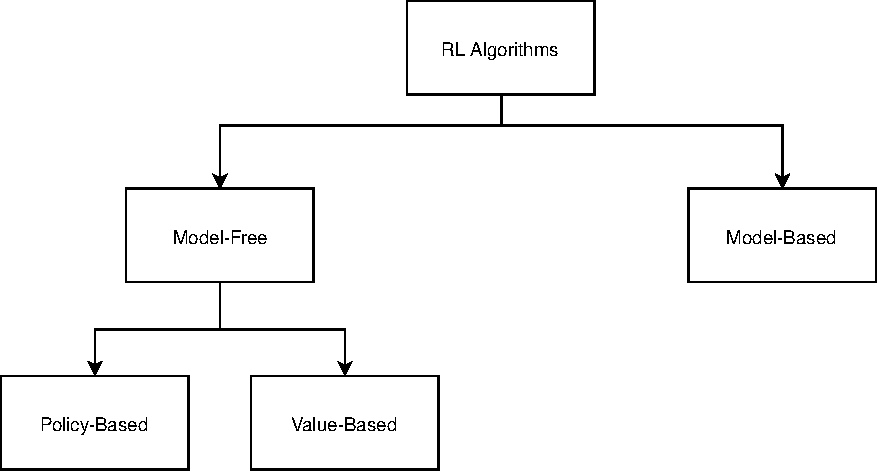
\includegraphics{images/rl_taxonomy}
  \caption[RL-Taxonomy]{Taxonomy of Reinforcement Learning algorithms. Source: Adapted from \cite{9418283}}
  \label{fig:rl_taxonomy}
\end{figure}  



\paragraph{Model-based}
Model-based methods require a model of the environment, hence, the agent has information regarding, how the environment will behave in various states and transitions. This information can be used to do \textit{planning}, i.e. predicting various situations in the future, without actually interacting with the environment. This is possible, due to the known state transition probability matrix, see \nameref{para:mdp}, \cite{richardsutton2018}.

\paragraph{Model-free}
The agent in model-free methods does not have a model of the environment. Therefore, by trial-and-error, the agent has to do \textit{learning}, i.e. learning which action maps to which state and which reward \cite{richardsutton2018}.

\paragraph{Policy-based}
In policy-based methods, a policy calculates the most optimal action in a given state. Thus, a policy $\pi$ can be seen as the distribution of a given state to all possible actions \cite{Arulkumaran_2017}:

\begin{equation}
\pi(a|s) = \mathbb{P}[A_{t} = a | S_{t} = s]
\label{eq:policy_pi}
\end{equation}

\paragraph{Value-based}
The value-based methods are using a value function to determine the benefit of being in a given state, i.e. the expected return for being in a given state is estimated. Starting in state $\mathnormal{s}$ and following policy $\pi$ afterwards, the estimation of the discounted return $\mathnormal{G}_{t}$ \cite{Arulkumaran_2017}. The state-value function can be formalized as following:

\begin{equation}
%V^\pi(s)=\mathbb{E}[R|s,\pi]
\mathrm{v}_{\pi}(s)=\mathbb{E}_{\pi}[G_t|S_t=s]
\label{eq:state_val_func}
\end{equation}

Similarly, the action-value function, or widelier known as the \textit{Q-function}, can also be used to calculate the expected return. The Q-function is the expected return when starting in state $\mathnormal{s}$, taking action $\mathnormal{a}$ and following policy $\pi$ afterwards \cite{Arulkumaran_2017}. Formalized as following:

\begin{equation}
%Q^\pi(s,a)=\mathbb{E}[R|s,a,\pi]
q_{\pi}(s,a)=\mathbb{E}_{\pi}[G_t|S_t=s,A_t=a]
\label{eq:state_val_func}
\end{equation}

\paragraph{Actor-critic}
Actor-critic methods are a combination of policy- and value-based methods. The policy is refered to as the \textit{actor} and the value function as the \textit{critic}. During training, the actor is receiving feedback from the cirtic on its performance, which it is using to improve its learning. In these methods, the critic is used as the baseline for the error calculation \cite{Arulkumaran_2017}, see \ref{ssec:q_learning}. 

\paragraph{On-policy}
In on-policy methods, the policy itself, that is making the decision for the next action to take, is either evaluated, or improved \cite{richardsutton2018}.

\paragraph{Off-policy}
Contrary to on-policy methods, off-policy methods do not evaluate, or improve, the policy, that is making the decision for the next action, but rather an additional policy, that is not used for action selection \cite{richardsutton2018}.

\paragraph{Exploration vs Exploitation}
In RL tasks, it is not a trivial to determine when an agent should focus on exploring the environment to possibly find eventually better actions and thus gain better rewards, or exploit the best known actions to maximize the return. Policies implement various strategies to tackle this trade-off. For instance, an $\epsilon$-greedy policy will select a random action with probability $\epsilon$ and will select the optimal action with probability $1 - \epsilon$. Initially, the probability of exploring the environment with an $\epsilon$-greedy policy is high, but it diminishes over time as more of the environment is explored. Another approach is a greedy policy, which will always select the action with the highest expected return \cite{richardsutton2018}.


\subsection{Q-Learning}
\label{ssec:q_learning}
Q-Learning is a value-based off-policy method that belongs to the family of Temporal Difference (TD) methods. These are basically model-free methods, that learn from raw experience and update their values based on estimates, rather than exact values. The Q-Learning method is defined by:
%\underbrace{{R_{t+1} + \gamma \max_{a} Q (S_{t+1}, a)}}_{\substack{\text{TD target value}}}
\begin{equation}
Q(s, a) \leftarrow Q(s, a) + \alpha \biggl[  \underbrace{{R_{t+1} + \gamma \max_{a'}  Q (s', a')}}_{\substack{\text{TD target}}} - \:Q (s, a)   \biggr]
\label{eq:q_learning}
\end{equation}

In this method, the Q-function directly approximates the optimal action-value function, without relying on the policy, that is being followed. Here, $\alpha$, is the \textit{learning rate}, which generally determines how much of the newly aquired information should be incooperated into the existing knowledgebase of a model. Essentially, this hyperparameter affects how fast an agent is learning. The equation within the brackets is a variation of the TD \textit{error}, which calculates the sum of the reward for the state transition $R_{t+1}$, the estimate of the current state $Q(s,a)$ and the optimal estimate of the successor state $\gamma \max_{a} Q (s', a')$. Calculating the difference between the estimate of a current and successor state is called bootstrapping \cite{richardsutton2018}.


\section{Deep Reinforcement Learning}

\subsection{Deep Q-Network}
\label{ssec:dqn}
\todo{Maybe better introduction}
The DQN by \citeA{mnih2015human} is based on the Q-Learning method, hence, it is a value-based off-policy method. It combines Reinforcement Learning with artificial neural networks. Initially, it was developed to play arcade games from the Atari 2600 console on an emulator, where the environment is the game itself, the state is the current frame of the game and an action was simply an action from all available actions of the game. DQN agents performed on human-like level or above in 29 of the 46 games, that were used for experiments \cite{mnih2015human}.  

The deep convolutional neural network is processing images by the size of 210 x 160 pixels with a 128-color palette. In an effort to enhance the capabilities and performance of the network, images are pre-processed, meaning the dimensions are downscaled to a single one (grey-scale) and cropped, so only the relevant area of the image is captured. Resulting in images with sizings of 84 x 84 pixels. In addition to those steps, four successive images are stacked, to obtain clearer information about the current state of the environment. A reason for this approach is that, when looking at a single frame, it is not clear, in which direction objects are moving to, or coming from. Hence, the decision to pre-process the data to 84 x 84 x 4 dimension input. The resulting input is then fed into the architecture depicted in figure \ref{fig:dqn_arch}.



\begin{figure}[H]
  \centering
  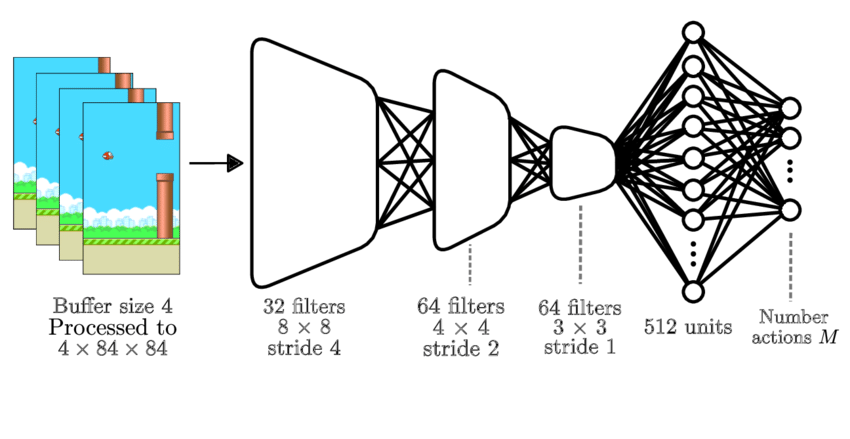
\includegraphics[scale=0.45]{images/dqn_arch}
  \caption[DQN Architecture]{DQN Architecture. The input data consists of four captured observations from the environment, that have been pre-processed into 84 x 84 dimensions. The input is successively passed into three hidden convolution layers, to extract and learn features from the observations. Each of the convolution layer is using rectified linear unit (ReLU) for the activation. Finally, the convoluted data is passed to the foruth hidden layer, which is fully-connected and consists of 512 rectifier units, followed by a fully-connected linear output layer, which has a mapping for each valid action in the environment. \protect\cite{mnih2015human}. Source: Reprinted from \protect\cite{Spears2017ScaleInvariant}}
  \label{fig:dqn_arch}
\end{figure}  



DQN agents use techniques such as Experience replay, fixed Q-targets, to learn the best action to take. In Experience replay, the experience of the agent, at each time step, is stored in a memory replay. \citeA{mnih2015human} stored tuples of $\langle S_t, A_t, R_{t+1}, S_{t+1} \rangle$, where $S_t$ is a stack of four images, to the memory in the Atari experiments. These experiences are collected at each timestep. Q-value updates are performed on a subset of the collected experience. The subset for the mini-batch training is selected random- and uniformly. The advantages of these approaches are, on the one hand, to increase the stability of the Q-network and, on the other hand, to increase the efficiency of the training, because correlation of successive experiences are removed \cite{richardsutton2018}.

The other technique, fixed Q-targets, uses an additional neural network with fixed parameters/weights \cite{silver2020DQN}. This neural network is called the target network and is initially a copy of the Q-network. However, during training, the weights of the target network are not updated, only those of the Q-network. They are frozen for most of the time and only updated with the Q-network weights after a certain number of training steps. Instead of using the Q-network as the target for the error calculation, this target network is used, hence the name.

\begin{equation}
\mathcal{L}_{i} (w_{i}) = \mathbb{E}_{(s,a,r,s')\sim \mathcal{D}_i} \Bigg[\bigg(    r+\gamma \max_{a'} Q(s',a';\theta_{i}^{-})-Q(s,a;\theta_{i} \bigg)^2\Bigg]
\label{eq:dqn_loss}
\end{equation}

The error, or loss, function for the DQN can be seen in equation \ref{eq:dqn_loss}. Here, $\mathcal{D}_i$, is the memory replay of the network, that consists of the previously mentioned experience tuples. Similar to the Q-learning method, the difference between the target and the current state is calculated. The difference to the Q-learning method, however, is that both Q-functions are parameterized policies, represented by the notations $\theta$. This implies that neural networks are utilized for estimating the Q-values. The dash in $\theta_{i}^{-}$ implies that the parameters, or weights, are fixed, i.e. the weights of this neural network are frozen and will not be updated. Freezing the weights of the target network results in an even more stable training of the Q-network.



\paragraph{Double Deep Q-Network}
\label{para:ddqn}
Double Deep Q-Network is an extention of the DQN. It addresses the issue that DQNs tend to select overestimated Q-values. This is due to the fact that the \textit{max} operator on the target Q-value is used for both, action selection and evaluation. Therefore, the selection of an action is decoupled from its evaluation \cite{van2016deep}. This results in the following formalization of the target network:

\begin{equation}
Y_{t}^{DoubleQ} = R_{t+1} + \gamma Q(s', \operatorname*{argmax}_a Q(s', a; \theta_{t}); \theta'_{t})
\label{eq:ddqn_target}
\end{equation}

Action selection is still due to $\theta_t$, however, the evaluation of the values is handled by the second neural network $\theta'_t$.




\subsection{REINFORCE}
\label{ssec:reinforce}
Although \citeA{williams1992simple} initially introduced REINFORCE as a class of methods, it now refers to a Monte-Carlo Policy Gradient method. It is, as the name implies, a policy-based method, that learns a parameterized policy. Monte Carlo methods, in the context of Reinforcement Learning, are methods that estimate the expected return by averaging the return from an entire episode. Consequently, parameterized policy-based methods are formalized by:

\begin{equation}
%\pi(a|s, \theta) = Pr\{A_{t} = a | S_{t} = s, \theta_t = \theta\}
\pi_{\theta}(s,a) = \mathbb{P} [a | s, \theta]
\label{eq:policy_parameterized}
\end{equation}

Policy gradient methods are methods that use the gradient of the objective function, $\mathrm{J}(\theta)$ (similar to the loss function in DQN), to find the optimal policy. In order to do this, a local maximum is explored during the gradient ascend of the policy. Formalized by:

\begin{equation}
%\theta_{t+1} = \theta_t +  \alpha \widehat{\nabla J(\theta_t)}
\Delta \theta = \alpha \nabla_{\theta} \mathrm{J}(\theta)
\label{eq:policy_gradient_descent}
\end{equation}

Here, $\alpha$, is the variable for the step-size and $\nabla_\theta J(\theta_t)$ is the policy gradient ($\nabla$ is symbolizing a gradient). $\Delta \theta$ represents the change of $\theta$, i.e. the updated weights \cite{richardsutton2018}.

Finally, the objective function in a policy gradient method can be formalized as following:

\begin{equation}
%\nabla J(\theta) = \mathbb{E}_\pi [G_t \nabla \ln{\pi} (A_t|S_t, \theta)]
\nabla_{\theta} \mathrm{J}(\theta) = \mathbb{E}_{\pi_{\theta}} [\nabla_{\theta}  \log \pi_{\theta} (s,a)\: Q^{\pi_{\theta}} (s, a)]
\label{eq:reinforce}
\end{equation}
 

\paragraph{Baseline}
Without altering the expectation, the variance can be decreased by subtracting a \textit{baseline} from the policy gradient. Subsequently, the state-value function is used as a baseline and subtracted from the Q-function, resulting in the advantage function $A^\mathrm{w}(s,a)$. A policy gradient with baseline is formalized by:
\begin{equation}
%\nabla J(\theta) = \mathbb{E}_\pi [(G_t - b(S_t)\nabla \ln{\pi} (A_t|S_t, \theta)]
\nabla_{\theta} \mathrm{J}(\theta) = \mathbb{E}_{\pi_{\theta}} [\nabla_{\theta}  \log \pi_{\theta} (s,a)\: A^{\pi_{\theta}} (s,a)]
\label{eq:reinforce_base}
\end{equation}





\subsection{Proximal Policy Optimization}
\label{ssec:ppo}

PPO by \citeA{schulman2017proximal} is another policy-based method. It is similar to the Trust Region Policy Optimization (TRPO) method by \citeA{schulman2015trust}. In TRPO, training stability is enhanced by constraining the extent to which a policy can be subjected to change at one step. The so-called \textit{trust region} prevents performance collapse, which may happen during policy updates with large step size updates. It is determined by calculating the Kullback-Leibler (KL) divergence between old and new policies at each iteration of a policy update. The KL divergence is a metric that shows how two probability distributions differ from one another . In TRPO the objective function is usually referred to as \textit{surrogate objective} \cite{schulman2015trust}.

%The KL divergence in TRPO is formalized by:

%\begin{equation}
%\mathbb{E}_{s \sim p^{\pi_{\theta_{old}}}} [D_{KL} (\pi_{\theta_{old}} (. |s) || \pi_\theta (. |s)) ] \leq \delta
%\label{eq:trpo_kldivergence}
%\end{equation}


PPO has the same aim as TRPO, maximizing the scope of the policy update in a single step without compromising the performance. Unlike TRPO, PPO uses less complex methods to achieve that goal, which makes it simpler to implement and easier to tune. There are two variations: PPO-Clip and PPO-Penalty.

\paragraph{PPO-Clip} In the PPO-Clip variant, the objective function is clipped and the KL divergence is not longer used. This is formalized by following equation:

\begin{equation}
L^{CLIP} (\theta) = \mathbb{\hat{{E}}}_t    \bigg[ min (r_t(\theta) \hat{A}_t, clip (r_t(\theta), 1-\epsilon, 1+\epsilon)\hat{A}_t) \bigg]
\label{eq:ppo_clipped}
\end{equation}

Here, $r_t(\theta)$, is the probability ratio between the old and new policy and $\hat{A}_t$ is an estimator at timestep $t$ of the advantage function. The hyperparameter $\epsilon$ controls how far the new policy can deviate from the old one, e.g. 0.2. By clipping the probability ratio and additionally applying the \textit{min}-operator to the original and clipped ratio, updates to the policy with large steps are omitted.

\paragraph{PPO-Penalty} The PPO-Penalty variant uses a penalty on the KL divergence. Each policy update iteration, this penalty coefficient is adapted to meet a target value. However, during the experiments by \citeA{schulman2017proximal}, this variant performed worse than the PPO-Clip variant and is only mentioned for completion.
